\documentclass{article}

\usepackage{fontspec}   %加這個就可以設定字體
\usepackage{xeCJK}       %讓中英文字體分開設置
\usepackage[T1]{fontenc}
\usepackage{bigfoot} % to allow verbatim in footnote
\usepackage[numbered,framed]{matlab-prettifier}
\usepackage{graphicx}
\usepackage{filecontents}
\graphicspath{ {img/} }
\setCJKmainfont{標楷體} %設定中文為系統上的字型,而英文不去更動,使用原TeX字型
\XeTeXlinebreaklocale "zh"             %這兩行一定要加,中文才能自動換行
\XeTeXlinebreakskip = 0pt plus 1pt     %這兩行一定要加,中文才能自動換行
\title{Introduction to Wireless and Mobile Networking\\ Homework \#3}
\author{B03901023 許秉鈞}
\date{April 30, 2017} %日期
\let\ph\mlplaceholder % shorter macro
\lstMakeShortInline"

\lstset{
  style              = Matlab-editor,
  basicstyle         = \mlttfamily,
  escapechar         = ",
  mlshowsectionrules = true,
}

\begin{document}
\maketitle

\begin{figure}[h]
    \centering
    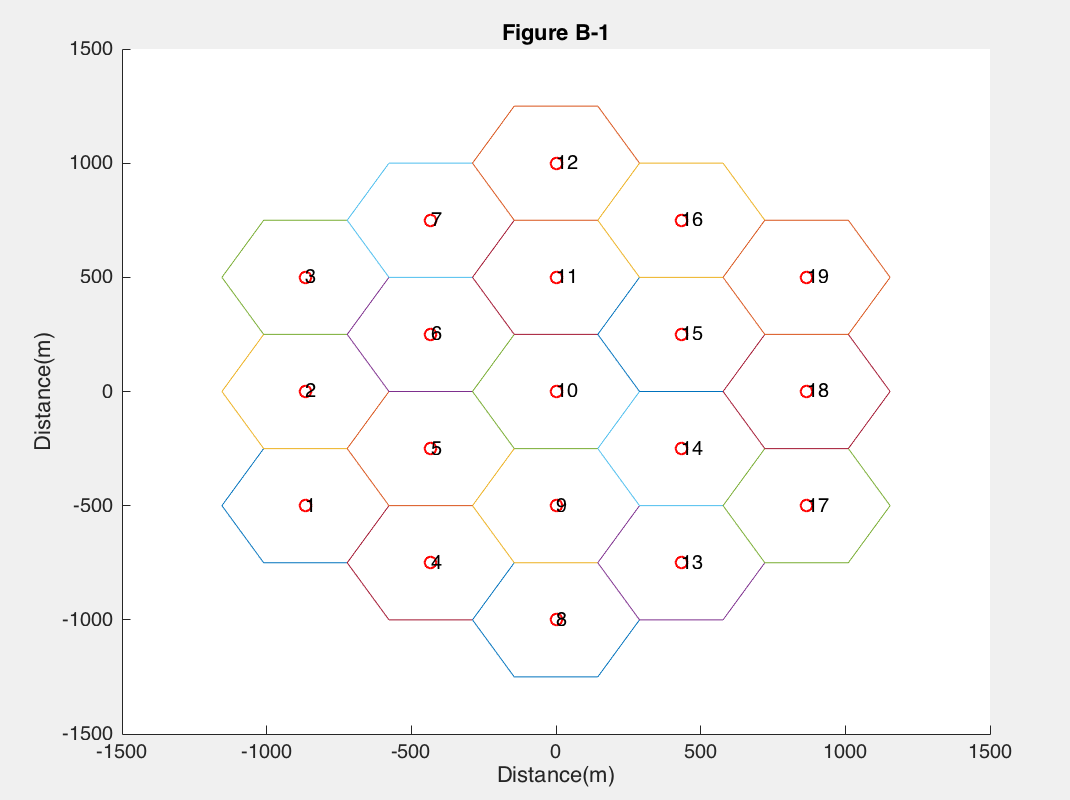
\includegraphics[width=1\textwidth]{fig1}
    \caption{\textit{Please give a figure to describe how you arrange cell IDs}}
    \label{fig:mesh1}
\end{figure}

\begin{figure}[h]
    \centering
    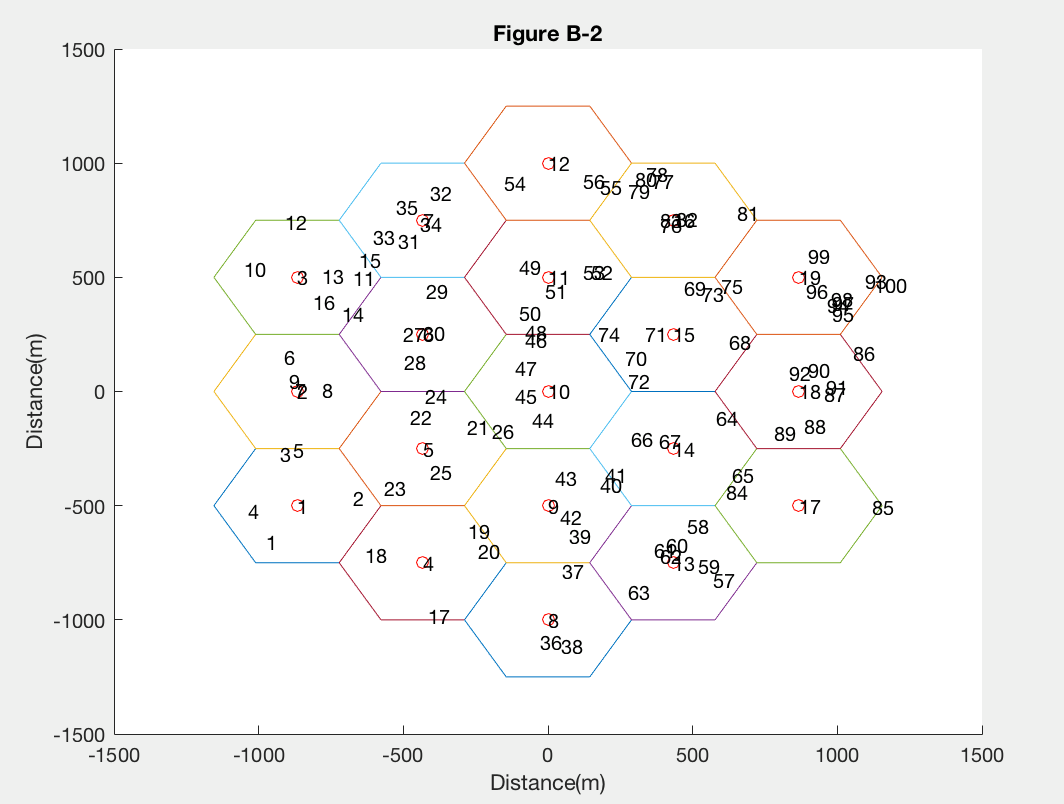
\includegraphics[width=1\textwidth]{fig2}
    \caption{\textit{Please plot a map with all mobile devices in their initial location}}
    \label{fig:mesh2}
\end{figure}

\begin{lstlisting}[caption = {rw\_mobile.m}]
classdef rw_mobile
    properties
        x
        y
        direction % a. moving direction between [0, 2pi] uniformly.
        speed % b. velocity between [minSpeed, maxSpeed] uniformly.
        time % c. moves t seconds, uniformly between [minT, maxT].
        label
    end
    properties(Constant = true)
        minSpeed = 1;
        maxSpeed = 15;
        minT = 1;
        maxT = 6;

        gt_db = 14;
        h_md = 1.5;
        p_ms_db = 23 - 30;
    end
    methods
        function obj = rw_mobile(x, y, direction, speed, time, label)
            if nargin == 6 % default value, use nargin
                obj.x = x;
                obj.y = y;
                obj.direction = direction;
                obj.speed = speed;
                obj.time = time;
                obj.label = label;
            else
                obj.x = 0;
                obj.y = 0;
                obj.direction = 0;
                obj.speed = 0;
                obj.time = 0;
                obj.label = 0;
            end
        end
        function[obj, x, y] = move(obj)
            obj.x = obj.x + obj.speed * cos(obj.direction);
            obj.y = obj.y + obj.speed * sin(obj.direction);
            obj.time = obj.time - 1;
            if obj.time <= 0
                obj.speed = unifrnd(obj.minSpeed, obj.maxSpeed);
                obj.direction = unifrnd(1, 2*pi);
                interval = obj.maxT - obj.minT;
                obj.time = obj.minT + unidrnd(interval);
            end
            x = obj.x;
            y = obj.y;
        end
        function obj = extend(obj, newX, newY)
            obj.x = newX;
            obj.y = newY;
        end
        function dist = getDist(obj, x_b, y_b)
            distX = obj.x - x_b;
            distY = obj.y - y_b;
            dist = sqrt(distX.^2 + distY.^2);
        end
        function [x,y] = getGeometry(obj)
            x = obj.x;
            y = obj.y;
        end
        function pow = getPower(obj, dist, hr, gr)
            gc = twoRayGnd(obj.h_md, hr, dist);
            pow = fromdB(obj.p_ms_db + obj.gt_db) * gc * gr;
        end
        function [obj, content] = getHandoff(obj, t, upper, content)
            if obj.label ~= upper
                prev = obj.label;
                obj.label = upper;
                len = size(content, 1);
                content(len + 1, :) = {strcat(int2str(t),'s'), prev, upper};
                fprintf('yes: %d\n', t);
            else
                fprintf('not: %d\n', t);
                prev = obj.label;
            end
        end
    end
end

\end{lstlisting}
\end{document}
